% Options for packages loaded elsewhere
\PassOptionsToPackage{unicode}{hyperref}
\PassOptionsToPackage{hyphens}{url}
\PassOptionsToPackage{dvipsnames,svgnames,x11names}{xcolor}
%
\documentclass[
  12pt,
]{article}
\usepackage{amsmath,amssymb}
\usepackage{lmodern}
\usepackage{iftex}
\ifPDFTeX
  \usepackage[T1]{fontenc}
  \usepackage[utf8]{inputenc}
  \usepackage{textcomp} % provide euro and other symbols
\else % if luatex or xetex
  \usepackage{unicode-math}
  \defaultfontfeatures{Scale=MatchLowercase}
  \defaultfontfeatures[\rmfamily]{Ligatures=TeX,Scale=1}
\fi
% Use upquote if available, for straight quotes in verbatim environments
\IfFileExists{upquote.sty}{\usepackage{upquote}}{}
\IfFileExists{microtype.sty}{% use microtype if available
  \usepackage[]{microtype}
  \UseMicrotypeSet[protrusion]{basicmath} % disable protrusion for tt fonts
}{}
\makeatletter
\@ifundefined{KOMAClassName}{% if non-KOMA class
  \IfFileExists{parskip.sty}{%
    \usepackage{parskip}
  }{% else
    \setlength{\parindent}{0pt}
    \setlength{\parskip}{6pt plus 2pt minus 1pt}}
}{% if KOMA class
  \KOMAoptions{parskip=half}}
\makeatother
\usepackage{xcolor}
\usepackage[margin=1in]{geometry}
\usepackage{longtable,booktabs,array}
\usepackage{calc} % for calculating minipage widths
% Correct order of tables after \paragraph or \subparagraph
\usepackage{etoolbox}
\makeatletter
\patchcmd\longtable{\par}{\if@noskipsec\mbox{}\fi\par}{}{}
\makeatother
% Allow footnotes in longtable head/foot
\IfFileExists{footnotehyper.sty}{\usepackage{footnotehyper}}{\usepackage{footnote}}
\makesavenoteenv{longtable}
\usepackage{graphicx}
\makeatletter
\def\maxwidth{\ifdim\Gin@nat@width>\linewidth\linewidth\else\Gin@nat@width\fi}
\def\maxheight{\ifdim\Gin@nat@height>\textheight\textheight\else\Gin@nat@height\fi}
\makeatother
% Scale images if necessary, so that they will not overflow the page
% margins by default, and it is still possible to overwrite the defaults
% using explicit options in \includegraphics[width, height, ...]{}
\setkeys{Gin}{width=\maxwidth,height=\maxheight,keepaspectratio}
% Set default figure placement to htbp
\makeatletter
\def\fps@figure{htbp}
\makeatother
\setlength{\emergencystretch}{3em} % prevent overfull lines
\providecommand{\tightlist}{%
  \setlength{\itemsep}{0pt}\setlength{\parskip}{0pt}}
\setcounter{secnumdepth}{5}
\usepackage{floatrow}
\floatsetup{capposition=top}
\usepackage{setspace}
\usepackage{fancyhdr}
\usepackage{titlesec}
\usepackage{geometry}
\usepackage{subfig}
\newcommand{\beginsupplement}{
\setcounter{table}{0}
\renewcommand{\thetable}{S\arabic{table}}
\setcounter{figure}{0}
\renewcommand{\thefigure}{S\arabic{figure}}}
\usepackage{booktabs}
\usepackage{longtable}
\usepackage{array}
\usepackage{multirow}
\usepackage{wrapfig}
\usepackage{float}
\usepackage{colortbl}
\usepackage{pdflscape}
\usepackage{tabu}
\usepackage{threeparttable}
\usepackage{threeparttablex}
\usepackage[normalem]{ulem}
\usepackage{makecell}
\usepackage{xcolor}
\ifLuaTeX
  \usepackage{selnolig}  % disable illegal ligatures
\fi
\IfFileExists{bookmark.sty}{\usepackage{bookmark}}{\usepackage{hyperref}}
\IfFileExists{xurl.sty}{\usepackage{xurl}}{} % add URL line breaks if available
\urlstyle{same} % disable monospaced font for URLs
\hypersetup{
  pdftitle={A Sociological Analysis of Structural Racism in `Student List' Lead Generation Products},
  pdfauthor={Ozan Jaquette; Karina G. Salazar},
  colorlinks=true,
  linkcolor={Maroon},
  filecolor={Maroon},
  citecolor={Blue},
  urlcolor={blue},
  pdfcreator={LaTeX via pandoc}}

\title{A Sociological Analysis of Structural Racism in `Student List' Lead Generation Products}
\author{Ozan Jaquette \and Karina G. Salazar}
\date{}

\begin{document}
\maketitle

\hypertarget{tables}{%
\section{Tables}\label{tables}}

\begin{table}[!h]

\caption{\label{tab:orders-filters-combo}Top filter combinations used in College Board orders purchased purchased by research vs. master's}
\centering
\resizebox{\linewidth}{!}{
\begin{tabular}[t]{lcclcc}
\toprule
\multicolumn{3}{c}{\textbf{Research}} & \multicolumn{3}{c}{\textbf{M.A.}} \\
\cmidrule(l{3pt}r{3pt}){1-3} \cmidrule(l{3pt}r{3pt}){4-6}
\textbf{Filters} & \textbf{Count} & \textbf{Percent} & \textbf{Filters} & \textbf{Count} & \textbf{Percent}\\
\midrule
HS grad class, GPA, SAT, Zip code & 99 & 19\% & HS grad class, GPA, PSAT, Zip code & 143 & 47\%\\
HS grad class, GPA, SAT, PSAT, Rank, State, Race & 39 & 7\% & HS grad class, GPA, SAT, Zip code & 107 & 35\%\\
HS grad class, SAT, State & 38 & 7\% & HS grad class, GPA, SAT, PSAT, Zip code & 28 & 9\%\\
HS grad class, PSAT, State & 28 & 5\% & HS grad class, SAT, Geomarket & 6 & 2\%\\
HS grad class, GPA, SAT, State & 23 & 4\% & HS grad class, GPA, SAT, PSAT, County & 4 & 1\%\\
\addlinespace
HS grad class, GPA, PSAT, State, Race & 20 & 4\% & HS grad class, GPA, SAT, County & 4 & 1\%\\
HS grad class, PSAT, State, Low SES & 20 & 4\% & HS grad class, SAT, Geomarket, College type & 2 & 1\%\\
HS grad class, GPA, PSAT, State & 19 & 4\% & HS grad class, PSAT, Geomarket & 2 & 1\%\\
HS grad class, GPA, AP score, Geomarket & 15 & 3\% & HS grad class, GPA, SAT, State, Segment, Major, Edu aspiration & 1 & 0\%\\
HS grad class, GPA, SAT, PSAT, State, Segment, Gender & 13 & 2\% & HS grad class, GPA, PSAT, State, Geomarket, Edu aspiration & 1 & 0\%\\
\bottomrule
\end{tabular}}
\end{table}

\emph{NOTES: Top filter combinations are based on 830 College Board student list purchases made by research (N=9) and master's (N=5) universities from 2016-2020. Geodemographic and Segment filters are proprietary filters created by College Board that use geodemography to predict the college-going behaviors of students within specific geographic areas.}

\clearpage

\newpage

\hypertarget{figures}{%
\section{Figures}\label{figures}}

Figure 1: College Entrance and Pre-Entrance Exam Filters Across Thresholds

(For Online Version)

\begin{itemize}
\tightlist
\item
  fig1\_p2sat\_inc.png
\item
  fig1\_p2sat\_exc.png
\item
  fig1\_p2psat\_inc.png
\item
  fig1\_p2psat\_exc.png
\item
  legend\_horizontal.png
\end{itemize}

(For Black and White Print Version)

\begin{itemize}
\tightlist
\item
  fig1\_p2sat\_inc\_bw.png
\item
  fig1\_p2sat\_exc\_bw.png
\item
  fig1\_p2psat\_inc\_bw.png
\item
  fig1\_p2psat\_exc\_bw.png
\item
  legend\_horizontal\_bw.png
\end{itemize}

SOURCE: U.S. Department of Education, National Center for Education Statistics, High School Longitudinal Study of 2009 (HSLS09).

\newpage

Figure 2: Zip Code Filter Across Affluence Percentiles

(For Online Version)

\begin{itemize}
\tightlist
\item
  fig2\_p3zip\_inc.png
\item
  fig2\_p3zip\_exc.png
\item
  legend\_horizontal.png
\end{itemize}

(For Black and White Print Version)

\begin{itemize}
\tightlist
\item
  fig2\_p3zip\_inc\_bw.png
\item
  fig2\_p3zip\_exc\_bw.png
\item
  legend\_horizontal\_bw.png
\end{itemize}

SOURCE: U.S. Department of Education, National Center for Education Statistics, High School Longitudinal Study of 2009 (HSLS09).

\pagebreak

Figure 3: Filters used in College Board Orders Purchased by 14 Public Universities \newline 

(For Online Version) \newline

\includegraphics{eepa_student_list_manuscript_figures_files/figure-latex/order-filters-empirical-report1-1.pdf}

\pagebreak

(For Print Version) \newline

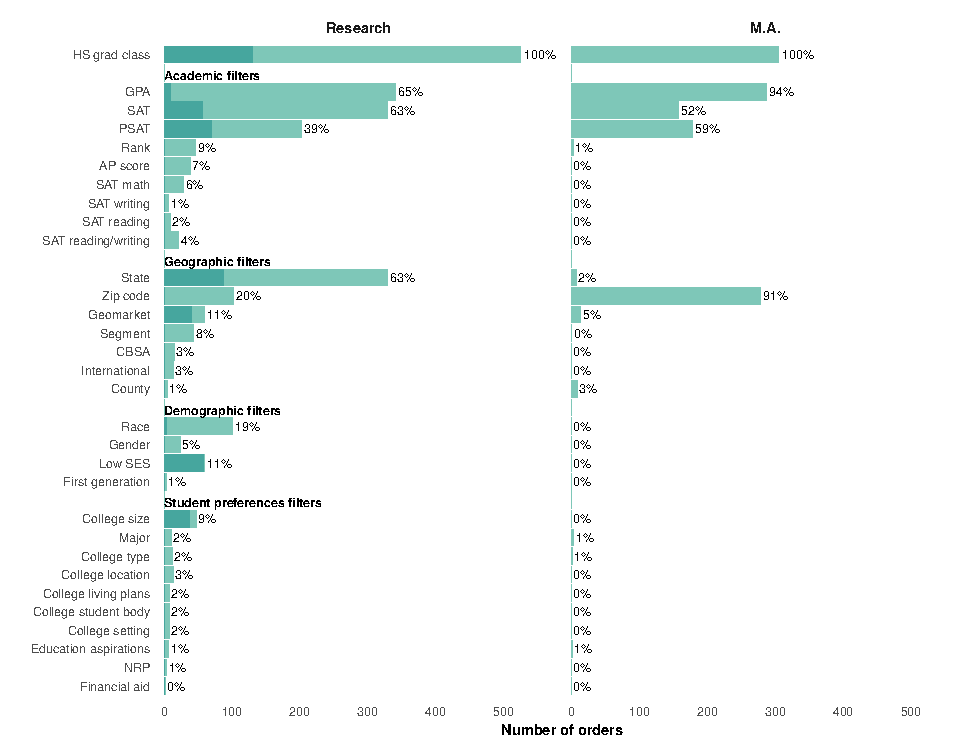
\includegraphics{eepa_student_list_manuscript_figures_files/figure-latex/order-filters-empirical-report-1.pdf}

NOTE: One research university placed a large amount of orders, which influenced the overall filters used for all research universities. The contribution of this particular university is shown in the darker color in the figure.

\pagebreak

Figure 4: SAT Filter Used by Research vs.~Master's Public Universities \newline

(Online Version) \newline
\includegraphics{eepa_student_list_manuscript_figures_files/figure-latex/orders-sat1-1.pdf}

(Print Version) \newline
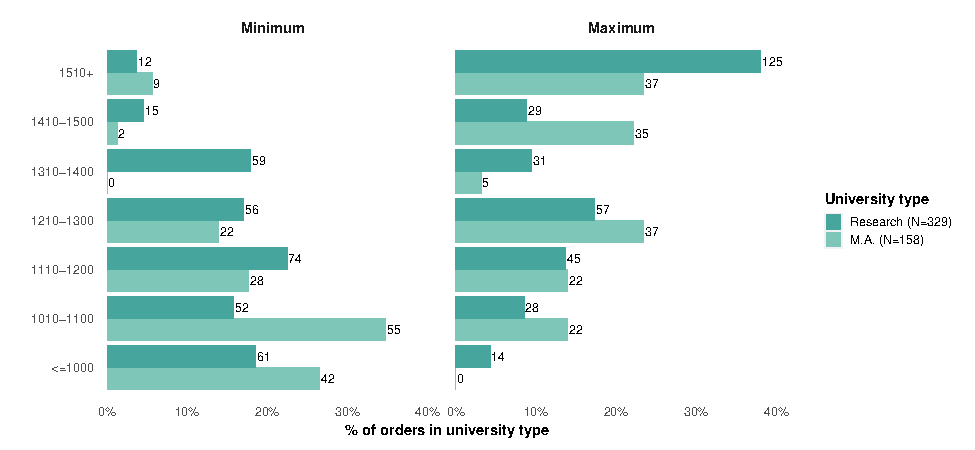
\includegraphics{eepa_student_list_manuscript_figures_files/figure-latex/orders-sat-1.pdf}

\pagebreak

Figure 5: Academic Combinations: GPA (3.0+) and College Entrance or Pre-Entrance Exams (across score thresholds)

(For Online Version)

\begin{itemize}
\tightlist
\item
  fig5\_combo1\_inc\_sat.png
\item
  fig5\_combo1\_inc\_psat.png
\item
  legend\_horizontal.png
\end{itemize}

(For Black and White Print Version)

\begin{itemize}
\tightlist
\item
  fig5\_combo1\_inc\_sat\_bw.png
\item
  fig5\_combo1\_inc\_psat\_bw.png
\item
  legend\_horizontal\_bw.png
\end{itemize}

SOURCE: U.S. Department of Education, National Center for Education Statistics, High School Longitudinal Study of 2009 (HSLS09).

\pagebreak

Figure 6: Academic and Geographic Combination: GPA (3.0+), College Pre-Entrance (150+) or Entrance (1050+) Exams, and Zip (across income thresholds)''

(For Online Version)

\begin{itemize}
\tightlist
\item
  fig6\_combo2\_inc\_sat.png
\item
  fig6\_combo2\_inc\_psat.png
\item
  legend\_horizontal.png
\end{itemize}

(For Black and White Print Version)

\begin{itemize}
\tightlist
\item
  fig6\_combo2\_inc\_sat\_bw.png
\item
  fig6\_combo2\_inc\_psat\_bw.png
\item
  legend\_horizontal\_bw.png
\end{itemize}

SOURCE: U.S. Department of Education, National Center for Education Statistics, High School Longitudinal Study of 2009 (HSLS09).

\pagebreak

Figure 7: Segment Filter Prospects by Metropolitan Area \newline 

(For Online Version) \newline
\includegraphics{eepa_student_list_manuscript_figures_files/figure-latex/uiuc-deep-dive1-1.pdf}

\pagebreak

(For Print Version) \newline
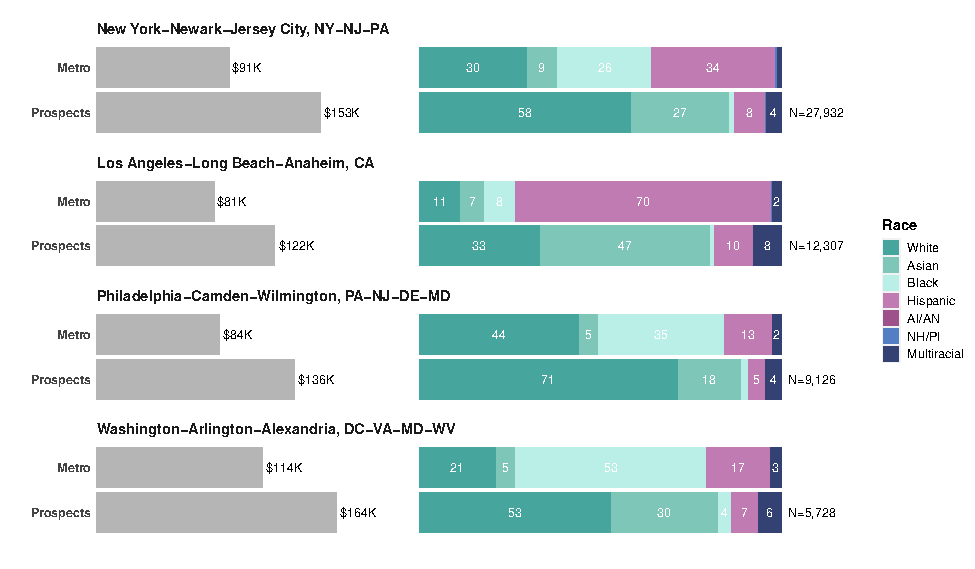
\includegraphics{eepa_student_list_manuscript_figures_files/figure-latex/uiuc-deep-dive-1.pdf}

\emph{Note: Filters used across these orders include HS Class, GPA (B-A+), State (in-state vs.~out-of-state), AP STEM (3 min for in-state; 4 min for out-of-state) or SAT (1200 minimum for in-state; 1300 minimum for out-of-state) with STEM major interest. Metro population source is the National Center for Education Statistic's Common Core of Data and includes all students attending a public high school in the metropolitan area. }

\pagebreak

Figure 8: Maps of Segment Filter Prospects by Metropolitan Area

(For Online Version)

\begin{itemize}
\tightlist
\item
  fig8\_map.png
\end{itemize}

(For Black and White Print Version)

\begin{itemize}
\tightlist
\item
  fig8\_map\_bw.png
\end{itemize}

\pagebreak

Figure 9: Women in STEM Prospects by Metropolitan Area \newline

(For Online Version) \newline
\includegraphics{eepa_student_list_manuscript_figures_files/figure-latex/ucsd-deep-dive1-1.pdf}

\pagebreak

(For Print Version) \newline
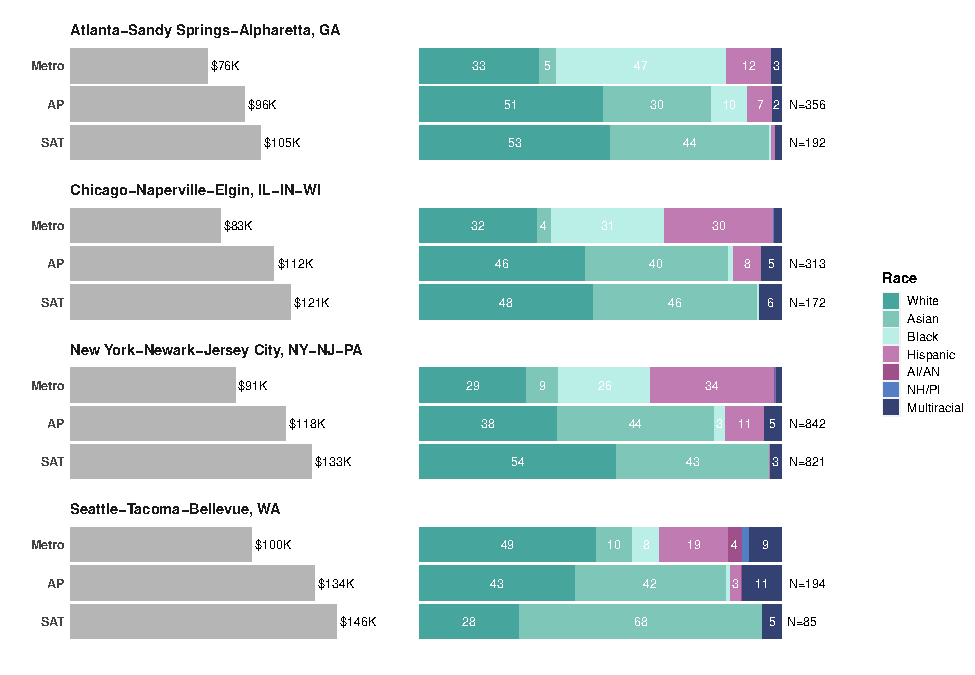
\includegraphics{eepa_student_list_manuscript_figures_files/figure-latex/ucsd-deep-dive-1.pdf}

\emph{Note: Filters used across these orders include HS Class, Segment, GPA (B-A+), PSAT/SAT (1220-1450); State/CBSAs. Metro population source is the National Center for Education Statistic's Common Core of Data and includes all students attending a public high school in the metropolitan area. }

\newpage

\hypertarget{supplemental-online-appendix}{%
\section{Supplemental Online Appendix}\label{supplemental-online-appendix}}

Figure S1: The Enrollment Funnel

\begin{itemize}
\tightlist
\item
  figs1\_enroll\_funnelv2.png
\end{itemize}

Figure S2: Test Takers Across College Extrance, College Pre-Entrance, and AP Assessments

\begin{itemize}
\tightlist
\item
  figS2\_p1\_sat.png
\item
  figS2\_p1\_ap.png
\item
  figS2\_p1\_psat.png
\item
  figS2\_p1\_apstem.png
\item
  legend\_horizontal.png
\end{itemize}

\begingroup
\fontsize{8}{8}\selectfont

SOURCE: U.S. Department of Education, National Center for Education Statistics, High School Longitudinal Study of 2009 (HSLS09).
\endgroup

Figure S3: AP Filter Across Thresholds

\begin{itemize}
\tightlist
\item
  figS3\_p2\_ap\_inc.png
\item
  figS3\_p2\_ap\_exc.png
\item
  figS3\_p2\_apstem\_inc.png
\item
  figS3\_p2\_apstem\_exc.png
\item
  legend\_horizontal.png
\end{itemize}

\begingroup
\fontsize{8}{8}\selectfont

SOURCE: U.S. Department of Education, National Center for Education Statistics, High School Longitudinal Study of 2009 (HSLS09).
\endgroup

\pagebreak

Figure S4: PSAT Filter Used by Research vs.~Master's Universities \newline

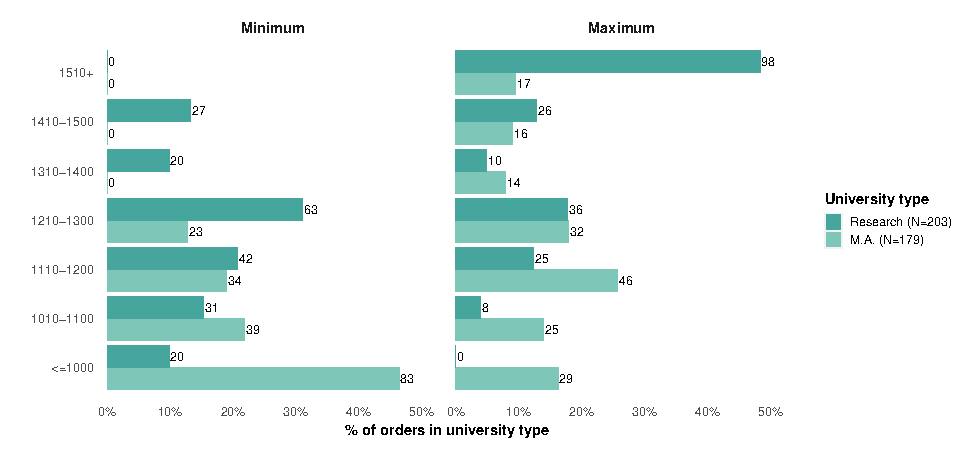
\includegraphics{eepa_student_list_manuscript_figures_files/figure-latex/orders-psat-1.pdf}

\pagebreak

Figure S5: Academic Combination: GPA (3.0+) and AP (across score thresholds)

\begin{itemize}
\tightlist
\item
  figS5\_combo3\_inc\_ap.png
\item
  figS5\_combo3\_inc\_apstem.png
\item
  legend\_horizontal.png
\end{itemize}

\begingroup
\fontsize{8}{8}\selectfont

SOURCE: U.S. Department of Education, National Center for Education Statistics, High School Longitudinal Study of 2009 (HSLS09).
\endgroup

\pagebreak

Table S1: HSLS09 Descriptive Statistics

\begin{table}[!h]
\centering\begingroup\fontsize{7}{9}\selectfont

\resizebox{\linewidth}{!}{
\begin{tabular}{lrrrr}
\toprule
\textbf{ } & \textbf{Unweighted} & \textbf{N} & \textbf{SE} & \textbf{Pct}\\
\midrule
\em{\textbf{Race/Ethnicity}} & \em{\textbf{}} & \em{\textbf{}} & \em{\textbf{}} & \em{\textbf{}}\\
White & 9,390 & 2,163,043 & 45,293 & 51.7\\
Asian & 1,370 & 150,222 & 15,373 & 3.6\\
Hisp & 2,520 & 920,384 & 41,451 & 22.0\\
Black & 1,660 & 574,370 & 36,346 & 13.7\\
Multi & 1,410 & 332,043 & 12,921 & 7.9\\
NH/PI & 70 & 18,784 & 5,241 & 0.4\\
AI/AN & 110 & 28,519 & 6,288 & 0.7\\
 &  &  &  & \\
\em{\textbf{Academic Filters}} & \em{\textbf{}} & \em{\textbf{}} & \em{\textbf{}} & \em{\textbf{}}\\
College Entrance Exam Completer & 7,910 & 1,860,677 & 54,277 & 55.6\\
College Pre-Entrance Exam Completer & 4,780 & 3,086,739 & 51,247 & 73.7\\
AP test-taker (any) & 2,990 & 694,359 & 33,918 & 16.6\\
AP test-taker (STEM) & 1,800 & 383,669 & 23,721 & 9.2\\
Academic GPA & 16,480 & 4,177,402 & 6,863 & 99.8\\
Missing Academic GPA & 40 & 9,964 & 6,562 & 0.2\\
\bottomrule
\end{tabular}}
\endgroup{}
\end{table}
\begingroup\fontsize{8}{12}\selectfont

\emph{NOTE: Unweighted sample sizes rounded to nearest 10 per NCES restricted data license regulations.}

\emph{SOURCE: U.S. Department of Education, National Center for Education
Statistics, High School Longitudinal Study of 2009 (HSLS09).}

\pagebreak

\landscape

Table S2: Characteristics of universities in public records request sample \newline

\begin{table}[!h]
\centering\begingroup\fontsize{3}{5}\selectfont

\resizebox{\linewidth}{!}{
\begin{tabular}{lrrrrrrrrrrr}
\toprule
\multicolumn{4}{c}{ } & \multicolumn{7}{c}{Undergraduate Freshmen} \\
\cmidrule(l{3pt}r{3pt}){5-11}
\begingroup\fontsize{2}{4}\selectfont \textbf{ }\endgroup & \begingroup\fontsize{2}{4}\selectfont \textbf{Type}\endgroup & \begingroup\fontsize{2}{4}\selectfont \textbf{Tuition \& Fees, In-State}\endgroup & \begingroup\fontsize{2}{4}\selectfont \textbf{Total Enrollment}\endgroup & \begingroup\fontsize{2}{4}\selectfont \textbf{\% Non-Resident}\endgroup & \begingroup\fontsize{2}{4}\selectfont \textbf{\% Pell}\endgroup & \begingroup\fontsize{2}{4}\selectfont \textbf{\% Asian}\endgroup & \begingroup\fontsize{2}{4}\selectfont \textbf{\% Black}\endgroup & \begingroup\fontsize{2}{4}\selectfont \textbf{\% Hispanic}\endgroup & \begingroup\fontsize{2}{4}\selectfont \textbf{\% Native American}\endgroup & \begingroup\fontsize{2}{4}\selectfont \textbf{\% Multiracial}\endgroup & \begingroup\fontsize{2}{4}\selectfont \textbf{\% White}\endgroup\\
\midrule
\cellcolor{gray!6}{Arizona State University-Tempe} & \cellcolor{gray!6}{Research} & \cellcolor{gray!6}{\$10,792} & \cellcolor{gray!6}{54,161} & \cellcolor{gray!6}{40} & \cellcolor{gray!6}{29} & \cellcolor{gray!6}{9} & \cellcolor{gray!6}{4} & \cellcolor{gray!6}{23} & \cellcolor{gray!6}{1} & \cellcolor{gray!6}{5} & \cellcolor{gray!6}{50}\\
Northern Arizona University & Research & \$10,289 & 29,609 & 38 & 35 & 2 & 3 & 26 & 2 & 7 & 57\\
\cellcolor{gray!6}{University of California-Davis} & \cellcolor{gray!6}{Research} & \cellcolor{gray!6}{\$14,419} & \cellcolor{gray!6}{31,437} & \cellcolor{gray!6}{19} & \cellcolor{gray!6}{33} & \cellcolor{gray!6}{25} & \cellcolor{gray!6}{2} & \cellcolor{gray!6}{23} & \cellcolor{gray!6}{0} & \cellcolor{gray!6}{5} & \cellcolor{gray!6}{21}\\
University of California-Irvine & Research & \$13,738 & 28,947 & 26 & 38 & 38 & 2 & 26 & 0 & 4 & 11\\
\cellcolor{gray!6}{University of California-San Diego} & \cellcolor{gray!6}{Research} & \cellcolor{gray!6}{\$14,018} & \cellcolor{gray!6}{29,613} & \cellcolor{gray!6}{26} & \cellcolor{gray!6}{31} & \cellcolor{gray!6}{34} & \cellcolor{gray!6}{1} & \cellcolor{gray!6}{23} & \cellcolor{gray!6}{0} & \cellcolor{gray!6}{5} & \cellcolor{gray!6}{18}\\
University of Illinois at Chicago & Research & \$15,027 & 19,476 & 8 & 59 & 22 & 8 & 40 & 0 & 3 & 22\\
\cellcolor{gray!6}{University of Illinois at Urbana-Champaign} & \cellcolor{gray!6}{Research} & \cellcolor{gray!6}{\$17,293} & \cellcolor{gray!6}{35,476} & \cellcolor{gray!6}{26} & \cellcolor{gray!6}{24} & \cellcolor{gray!6}{20} & \cellcolor{gray!6}{7} & \cellcolor{gray!6}{13} & \cellcolor{gray!6}{0} & \cellcolor{gray!6}{3} & \cellcolor{gray!6}{41}\\
Illinois State University & Research & \$12,353 & 20,115 & 4 & 30 & 2 & 10 & 12 & 0 & 3 & 71\\
\cellcolor{gray!6}{Northeastern Illinois University} & \cellcolor{gray!6}{Master's} & \cellcolor{gray!6}{\$9,638} & \cellcolor{gray!6}{9,260} & \cellcolor{gray!6}{2} & \cellcolor{gray!6}{64} & \cellcolor{gray!6}{6} & \cellcolor{gray!6}{30} & \cellcolor{gray!6}{44} & \cellcolor{gray!6}{0} & \cellcolor{gray!6}{2} & \cellcolor{gray!6}{11}\\
University of Illinois at Springfield & Master's & \$11,523 & 3,500 & 10 & 38 & 2 & 18 & 18 & 1 & 5 & 52\\
\cellcolor{gray!6}{Texas A\&M University-Texarkana} & \cellcolor{gray!6}{Master's} & \cellcolor{gray!6}{\$6,963} & \cellcolor{gray!6}{1,953} & \cellcolor{gray!6}{16} & \cellcolor{gray!6}{42} & \cellcolor{gray!6}{1} & \cellcolor{gray!6}{16} & \cellcolor{gray!6}{23} & \cellcolor{gray!6}{0} & \cellcolor{gray!6}{4} & \cellcolor{gray!6}{46}\\
Stephen F Austin State University & Master's & \$7,716 & 12,149 & 1 & 41 & 1 & 16 & 24 & 0 & 5 & 53\\
\cellcolor{gray!6}{Tarleton State University} & \cellcolor{gray!6}{Master's} & \cellcolor{gray!6}{\$7,367} & \cellcolor{gray!6}{12,853} & \cellcolor{gray!6}{2} & \cellcolor{gray!6}{40} & \cellcolor{gray!6}{1} & \cellcolor{gray!6}{6} & \cellcolor{gray!6}{21} & \cellcolor{gray!6}{0} & \cellcolor{gray!6}{3} & \cellcolor{gray!6}{67}\\
Texas A \& M University-College Station & Research & \$10,294 & 53,515 & 6 & 21 & 9 & 3 & 26 & 0 & 3 & 58\\
\bottomrule
\end{tabular}}
\endgroup{}
\end{table}
\begingroup
\fontsize{10}{10}\selectfont

\emph{SOURCE: U.S. Department of Education, Integrated Postsecondary Education Data System, 2017-18.}
\endgroup

\pagebreak
\endlandscape

Table S3: Assessment Completer Differences in Proportion

\begin{table}[!h]
\centering\begingroup\fontsize{2.5}{4.5}\selectfont

\resizebox{\linewidth}{!}{
\begin{tabular}{lrrrrr}
\toprule
\begingroup\fontsize{2}{4}\selectfont \textbf{ }\endgroup & \begingroup\fontsize{2}{4}\selectfont \textbf{Included}\endgroup & \begingroup\fontsize{2}{4}\selectfont \textbf{Excluded}\endgroup & \begingroup\fontsize{2}{4}\selectfont \textbf{Difference}\endgroup & \begingroup\fontsize{2}{4}\selectfont \textbf{Lower CI}\endgroup & \begingroup\fontsize{2}{4}\selectfont \textbf{Upper CI}\endgroup\\
\midrule
\addlinespace[0.3em]
\multicolumn{6}{l}{\textbf{College Entrance Exam}}\\
\cellcolor{gray!6}{\hspace{1em}White} & \cellcolor{gray!6}{0.573} & \cellcolor{gray!6}{0.472} & \cellcolor{gray!6}{0.101***} & \cellcolor{gray!6}{0.100} & \cellcolor{gray!6}{0.102}\\
\hspace{1em}Asian & 0.045 & 0.029 & 0.016*** & 0.015 & 0.016\\
\cellcolor{gray!6}{\hspace{1em}Hisp} & \cellcolor{gray!6}{0.173} & \cellcolor{gray!6}{0.257} & \cellcolor{gray!6}{-0.084***} & \cellcolor{gray!6}{-0.085} & \cellcolor{gray!6}{-0.083}\\
\hspace{1em}Black & 0.124 & 0.147 & -0.023*** & -0.024 & -0.022\\
\cellcolor{gray!6}{\hspace{1em}Multi} & \cellcolor{gray!6}{0.077} & \cellcolor{gray!6}{0.081} & \cellcolor{gray!6}{-0.004***} & \cellcolor{gray!6}{-0.005} & \cellcolor{gray!6}{-0.004}\\
\hspace{1em}NH/PI & 0.003 & 0.006 & -0.003*** & -0.003 & -0.002\\
\cellcolor{gray!6}{\hspace{1em}AI/AN} & \cellcolor{gray!6}{0.005} & \cellcolor{gray!6}{0.008} & \cellcolor{gray!6}{-0.003***} & \cellcolor{gray!6}{-0.003} & \cellcolor{gray!6}{-0.003}\\
\addlinespace[0.3em]
\multicolumn{6}{l}{\textbf{College Pre-Entrance Exam}}\\
\hspace{1em}White & 0.533 & 0.511 & 0.022*** & 0.021 & 0.023\\
\cellcolor{gray!6}{\hspace{1em}Asian} & \cellcolor{gray!6}{0.058} & \cellcolor{gray!6}{0.028} & \cellcolor{gray!6}{0.030***} & \cellcolor{gray!6}{0.030} & \cellcolor{gray!6}{0.031}\\
\hspace{1em}Hisp & 0.199 & 0.227 & -0.028*** & -0.029 & -0.027\\
\cellcolor{gray!6}{\hspace{1em}Black} & \cellcolor{gray!6}{0.125} & \cellcolor{gray!6}{0.142} & \cellcolor{gray!6}{-0.017***} & \cellcolor{gray!6}{-0.018} & \cellcolor{gray!6}{-0.016}\\
\hspace{1em}Multi & 0.08 & 0.079 & 0.001*** & 0.001 & 0.002\\
\cellcolor{gray!6}{\hspace{1em}NH/PI} & \cellcolor{gray!6}{0.003} & \cellcolor{gray!6}{0.005} & \cellcolor{gray!6}{-0.002***} & \cellcolor{gray!6}{-0.002} & \cellcolor{gray!6}{-0.002}\\
\hspace{1em}AI/AN & 0.002 & 0.009 & -0.007*** & -0.007 & -0.007\\
\addlinespace[0.3em]
\multicolumn{6}{l}{\textbf{AP}}\\
\cellcolor{gray!6}{\hspace{1em}White} & \cellcolor{gray!6}{0.542} & \cellcolor{gray!6}{0.512} & \cellcolor{gray!6}{0.030***} & \cellcolor{gray!6}{0.029} & \cellcolor{gray!6}{0.031}\\
\hspace{1em}Asian & 0.083 & 0.026 & 0.057*** & 0.056 & 0.058\\
\cellcolor{gray!6}{\hspace{1em}Hisp} & \cellcolor{gray!6}{0.216} & \cellcolor{gray!6}{0.221} & \cellcolor{gray!6}{-0.005***} & \cellcolor{gray!6}{-0.006} & \cellcolor{gray!6}{-0.004}\\
\hspace{1em}Black & 0.081 & 0.148 & -0.067*** & -0.068 & -0.067\\
\cellcolor{gray!6}{\hspace{1em}Multi} & \cellcolor{gray!6}{0.072} & \cellcolor{gray!6}{0.081} & \cellcolor{gray!6}{-0.009***} & \cellcolor{gray!6}{-0.009} & \cellcolor{gray!6}{-0.008}\\
\hspace{1em}NH/PI & 0.005 & 0.004 & 0.001*** & 0.000 & 0.001\\
\cellcolor{gray!6}{\hspace{1em}AI/AN} & \cellcolor{gray!6}{0.001} & \cellcolor{gray!6}{0.008} & \cellcolor{gray!6}{-0.007***} & \cellcolor{gray!6}{-0.007} & \cellcolor{gray!6}{-0.006}\\
\addlinespace[0.3em]
\multicolumn{6}{l}{\textbf{AP STEM}}\\
\hspace{1em}White & 0.557 & 0.513 & 0.044*** & 0.043 & 0.046\\
\cellcolor{gray!6}{\hspace{1em}Asian} & \cellcolor{gray!6}{0.11} & \cellcolor{gray!6}{0.028} & \cellcolor{gray!6}{0.082***} & \cellcolor{gray!6}{0.081} & \cellcolor{gray!6}{0.083}\\
\hspace{1em}Hisp & 0.193 & 0.223 & -0.030*** & -0.031 & -0.029\\
\cellcolor{gray!6}{\hspace{1em}Black} & \cellcolor{gray!6}{0.074} & \cellcolor{gray!6}{0.144} & \cellcolor{gray!6}{-0.070***} & \cellcolor{gray!6}{-0.071} & \cellcolor{gray!6}{-0.069}\\
\hspace{1em}Multi & 0.06 & 0.081 & -0.021*** & -0.022 & -0.020\\
\cellcolor{gray!6}{\hspace{1em}NH/PI} & \cellcolor{gray!6}{0.004} & \cellcolor{gray!6}{0.005} & \cellcolor{gray!6}{-0.001} & \cellcolor{gray!6}{-0.000} & \cellcolor{gray!6}{0.000}\\
\hspace{1em}AI/AN & 0.002 & 0.007 & -0.005*** & -0.006 & -0.005\\
\bottomrule
\end{tabular}}
\endgroup{}
\end{table}
\begingroup
\fontsize{10}{10}\selectfont

\emph{NOTE: \texttt{*}p\textless0.05, \texttt{**}p\textless0.01, \texttt{***}p\textless0.001}

\emph{SOURCE: U.S. Department of Education, National Center for Education Statistics, High School Longitudinal Study of 2009 (HSLS09).}
\endgroup

\pagebreak

Table S4: Score Threshold Proportion Differences in Included vs.~Excluded across Race/Ethnicity

\begin{table}[!h]
\centering\begingroup\fontsize{4}{6}\selectfont

\resizebox{\linewidth}{!}{
\begin{tabular}{lrrrrrrr}
\toprule
\begingroup\fontsize{6}{8}\selectfont \textbf{ }\endgroup & \begingroup\fontsize{6}{8}\selectfont \textbf{White}\endgroup & \begingroup\fontsize{6}{8}\selectfont \textbf{Asian}\endgroup & \begingroup\fontsize{6}{8}\selectfont \textbf{Hisp}\endgroup & \begingroup\fontsize{6}{8}\selectfont \textbf{Black}\endgroup & \begingroup\fontsize{6}{8}\selectfont \textbf{Multi}\endgroup & \begingroup\fontsize{6}{8}\selectfont \textbf{NH/PI}\endgroup & \begingroup\fontsize{6}{8}\selectfont \textbf{AI/AN}\endgroup\\
\midrule
\addlinespace[0.3em]
\multicolumn{8}{l}{\textbf{College Entrance Exam}}\\
\cellcolor{gray!6}{\hspace{1em}Less than 1000} & \cellcolor{gray!6}{-0.062***} & \cellcolor{gray!6}{-0.010***} & \cellcolor{gray!6}{0.004***} & \cellcolor{gray!6}{0.065***} & \cellcolor{gray!6}{0.005***} & \cellcolor{gray!6}{-0.003***} & \cellcolor{gray!6}{0.002***}\\
\hspace{1em}1000+ & 0.217*** & 0.033*** & -0.129*** & -0.103*** & -0.012*** & -0.001*** & -0.006***\\
\cellcolor{gray!6}{\hspace{1em}1200+} & \cellcolor{gray!6}{0.209***} & \cellcolor{gray!6}{0.057***} & \cellcolor{gray!6}{-0.137***} & \cellcolor{gray!6}{-0.103***} & \cellcolor{gray!6}{-0.025***} & \cellcolor{gray!6}{0.001***} & \cellcolor{gray!6}{-0.003***}\\
\hspace{1em}1300+ & 0.205*** & 0.090*** & -0.137*** & -0.122*** & -0.027*** & -0.002*** & NA\\
\cellcolor{gray!6}{\hspace{1em}1400+} & \cellcolor{gray!6}{0.170***} & \cellcolor{gray!6}{0.160***} & \cellcolor{gray!6}{-0.175***} & \cellcolor{gray!6}{-0.130***} & \cellcolor{gray!6}{-0.012***} & \cellcolor{gray!6}{NA} & \cellcolor{gray!6}{NA}\\
\addlinespace[0.3em]
\multicolumn{8}{l}{\textbf{College Pre-Entrance Exam}}\\
\hspace{1em}Less than 120 & -0.194*** & 0.007*** & 0.076*** & 0.105*** & 0.014*** & -0.004*** & -0.005***\\
\cellcolor{gray!6}{\hspace{1em}120+} & \cellcolor{gray!6}{0.098***} & \cellcolor{gray!6}{0.034***} & \cellcolor{gray!6}{-0.062***} & \cellcolor{gray!6}{-0.060***} & \cellcolor{gray!6}{-0.003***} & \cellcolor{gray!6}{-0.001***} & \cellcolor{gray!6}{-0.006***}\\
\hspace{1em}170+ & 0.185*** & 0.051*** & -0.093*** & -0.123*** & -0.015*** & 0.001* & NA\\
\cellcolor{gray!6}{\hspace{1em}200+} & \cellcolor{gray!6}{0.116***} & \cellcolor{gray!6}{0.151***} & \cellcolor{gray!6}{-0.102***} & \cellcolor{gray!6}{NA} & \cellcolor{gray!6}{-0.015***} & \cellcolor{gray!6}{NA} & \cellcolor{gray!6}{NA}\\
\hspace{1em}220+ & -0.078*** & 0.417*** & -0.191*** & NA & 0.002 & NA & NA\\
\addlinespace[0.3em]
\multicolumn{8}{l}{\textbf{AP}}\\
\cellcolor{gray!6}{\hspace{1em}1} & \cellcolor{gray!6}{-0.143***} & \cellcolor{gray!6}{0.022***} & \cellcolor{gray!6}{0.056***} & \cellcolor{gray!6}{0.077***} & \cellcolor{gray!6}{-0.001} & \cellcolor{gray!6}{-0.003***} & \cellcolor{gray!6}{-0.006***}\\
\hspace{1em}2+ & 0.066*** & 0.061*** & -0.017*** & -0.094*** & -0.010*** & 0.001*** & -0.007***\\
\cellcolor{gray!6}{\hspace{1em}3+} & \cellcolor{gray!6}{0.070***} & \cellcolor{gray!6}{0.058***} & \cellcolor{gray!6}{-0.017***} & \cellcolor{gray!6}{-0.091***} & \cellcolor{gray!6}{-0.015***} & \cellcolor{gray!6}{0.001*} & \cellcolor{gray!6}{-0.005***}\\
\hspace{1em}4+ & 0.086*** & 0.071*** & -0.022*** & -0.106*** & -0.026*** & 0.003*** & -0.005***\\
\cellcolor{gray!6}{\hspace{1em}5+} & \cellcolor{gray!6}{0.084***} & \cellcolor{gray!6}{0.104***} & \cellcolor{gray!6}{-0.046***} & \cellcolor{gray!6}{-0.109***} & \cellcolor{gray!6}{-0.025***} & \cellcolor{gray!6}{0.001} & \cellcolor{gray!6}{NA}\\
\addlinespace[0.3em]
\multicolumn{8}{l}{\textbf{AP STEM}}\\
\hspace{1em}1 & -0.100*** & 0.046*** & 0.090*** & 0.015*** & -0.040*** & -0.004*** & -0.007***\\
\cellcolor{gray!6}{\hspace{1em}2+} & \cellcolor{gray!6}{0.101***} & \cellcolor{gray!6}{0.092***} & \cellcolor{gray!6}{-0.077***} & \cellcolor{gray!6}{-0.101***} & \cellcolor{gray!6}{-0.012***} & \cellcolor{gray!6}{0.002***} & \cellcolor{gray!6}{-0.005***}\\
\hspace{1em}3+ & 0.130*** & 0.105*** & -0.097*** & -0.111*** & -0.025*** & 0.003*** & -0.005***\\
\cellcolor{gray!6}{\hspace{1em}4+} & \cellcolor{gray!6}{0.113***} & \cellcolor{gray!6}{0.119***} & \cellcolor{gray!6}{-0.106***} & \cellcolor{gray!6}{-0.103***} & \cellcolor{gray!6}{-0.023***} & \cellcolor{gray!6}{0.007***} & \cellcolor{gray!6}{-0.006***}\\
\hspace{1em}5+ & 0.078*** & 0.151*** & -0.101*** & -0.096*** & -0.020*** & NA & NA\\
\addlinespace[0.3em]
\multicolumn{8}{l}{\textbf{GPA}}\\
\cellcolor{gray!6}{\hspace{1em}Less than 2.0} & \cellcolor{gray!6}{-0.198***} & \cellcolor{gray!6}{-0.036***} & \cellcolor{gray!6}{0.104***} & \cellcolor{gray!6}{0.109***} & \cellcolor{gray!6}{0.016***} & \cellcolor{gray!6}{-0.002***} & \cellcolor{gray!6}{0.006***}\\
\hspace{1em}2.0+ & 0.193*** & 0.037*** & -0.103*** & -0.107*** & -0.016*** & 0.002*** & -0.006***\\
\cellcolor{gray!6}{\hspace{1em}2.5+} & \cellcolor{gray!6}{0.212***} & \cellcolor{gray!6}{0.037***} & \cellcolor{gray!6}{-0.112***} & \cellcolor{gray!6}{-0.112***} & \cellcolor{gray!6}{-0.018***} & \cellcolor{gray!6}{-0.001***} & \cellcolor{gray!6}{-0.006***}\\
\hspace{1em}3.0+ & 0.109*** & 0.032*** & -0.068*** & -0.060*** & -0.008*** & -0.004*** & -0.002***\\
\cellcolor{gray!6}{\hspace{1em}3.5+} & \cellcolor{gray!6}{0.233***} & \cellcolor{gray!6}{0.034***} & \cellcolor{gray!6}{-0.124***} & \cellcolor{gray!6}{-0.112***} & \cellcolor{gray!6}{-0.026***} & \cellcolor{gray!6}{0.000} & \cellcolor{gray!6}{-0.006***}\\
\bottomrule
\end{tabular}}
\endgroup{}
\end{table}

\begingroup
\fontsize{10}{10}\selectfont

\emph{NOTE: \texttt{*}p\textless0.05, \texttt{**}p\textless0.01, \texttt{***}p\textless0.001}

\emph{SOURCE: U.S. Department of Education, National Center for Education Statistics, High School Longitudinal Study of 2009 (HSLS09).}
\endgroup

\pagebreak

Table S5: Zip Code Affluence Proportion Differences in Included vs.~Excluded across Race/Ethnicity

\begin{table}[!h]
\centering\begingroup\fontsize{4}{6}\selectfont

\resizebox{\linewidth}{!}{
\begin{tabular}{lrrrrrrr}
\toprule
\begingroup\fontsize{6}{8}\selectfont \textbf{ }\endgroup & \begingroup\fontsize{6}{8}\selectfont \textbf{White}\endgroup & \begingroup\fontsize{6}{8}\selectfont \textbf{Asian}\endgroup & \begingroup\fontsize{6}{8}\selectfont \textbf{Hisp}\endgroup & \begingroup\fontsize{6}{8}\selectfont \textbf{Black}\endgroup & \begingroup\fontsize{6}{8}\selectfont \textbf{Multi}\endgroup & \begingroup\fontsize{6}{8}\selectfont \textbf{NH/PI}\endgroup & \begingroup\fontsize{6}{8}\selectfont \textbf{AI/AN}\endgroup\\
\midrule
\addlinespace[0.3em]
\multicolumn{8}{l}{\textbf{Affluence Percentile}}\\
\cellcolor{gray!6}{\hspace{1em}Less than 20\%} & \cellcolor{gray!6}{-0.248***} & \cellcolor{gray!6}{-0.009***} & \cellcolor{gray!6}{0.112***} & \cellcolor{gray!6}{0.156***} & \cellcolor{gray!6}{-0.008***} & \cellcolor{gray!6}{0.001***} & \cellcolor{gray!6}{-0.003***}\\
\hspace{1em}20-39\% & -0.030*** & -0.011*** & 0.034*** & -0.005*** & 0.008*** & -0.004*** & 0.008***\\
\cellcolor{gray!6}{\hspace{1em}40-59\%} & \cellcolor{gray!6}{0.035***} & \cellcolor{gray!6}{-0.014***} & \cellcolor{gray!6}{0.015***} & \cellcolor{gray!6}{-0.028***} & \cellcolor{gray!6}{-0.005***} & \cellcolor{gray!6}{-0.002***} & \cellcolor{gray!6}{0.000}\\
\hspace{1em}60-79\% & 0.051*** & -0.004*** & -0.035*** & -0.024*** & 0.011*** & 0.004*** & -0.003***\\
\cellcolor{gray!6}{\hspace{1em}80-89\%} & \cellcolor{gray!6}{0.079***} & \cellcolor{gray!6}{0.000*} & \cellcolor{gray!6}{-0.028***} & \cellcolor{gray!6}{-0.054***} & \cellcolor{gray!6}{0.001*} & \cellcolor{gray!6}{0.002***} & \cellcolor{gray!6}{0.000***}\\
\hspace{1em}Greater than 90\% & 0.151*** & 0.047*** & -0.108*** & -0.071*** & -0.013*** & 0.001*** & -0.004***\\
\bottomrule
\end{tabular}}
\endgroup{}
\end{table}

\begingroup
\fontsize{10}{10}\selectfont

\emph{NOTE: \texttt{*}p\textless0.05, \texttt{**}p\textless0.01, \texttt{***}p\textless0.001}

\emph{SOURCE: U.S. Department of Education, National Center for Education Statistics, High School Longitudinal Study of 2009 (HSLS09).}
\endgroup

\clearpage

Table S6: GPA and College Entrance or Pre-Entrance Exam Score Threshold Proportion Differences in Included vs.~Excluded across Race/Ethnicity

\begin{table}[!h]
\centering\begingroup\fontsize{4}{6}\selectfont

\resizebox{\linewidth}{!}{
\begin{tabular}{lrrrrrrr}
\toprule
\begingroup\fontsize{6}{8}\selectfont \textbf{ }\endgroup & \begingroup\fontsize{6}{8}\selectfont \textbf{White}\endgroup & \begingroup\fontsize{6}{8}\selectfont \textbf{Asian}\endgroup & \begingroup\fontsize{6}{8}\selectfont \textbf{Hisp}\endgroup & \begingroup\fontsize{6}{8}\selectfont \textbf{Black}\endgroup & \begingroup\fontsize{6}{8}\selectfont \textbf{Multi}\endgroup & \begingroup\fontsize{6}{8}\selectfont \textbf{NH/PI}\endgroup & \begingroup\fontsize{6}{8}\selectfont \textbf{AI/AN}\endgroup\\
\midrule
\addlinespace[0.3em]
\multicolumn{8}{l}{\textbf{College Entrance Exam}}\\
\cellcolor{gray!6}{\hspace{1em}1050+} & \cellcolor{gray!6}{0.233***} & \cellcolor{gray!6}{0.041***} & \cellcolor{gray!6}{-0.133***} & \cellcolor{gray!6}{-0.124***} & \cellcolor{gray!6}{-0.011***} & \cellcolor{gray!6}{0.001} & \cellcolor{gray!6}{-0.006***}\\
\hspace{1em}1100+ & 0.229*** & 0.045*** & -0.127*** & -0.130*** & -0.011*** & -0.002*** & -0.004***\\
\cellcolor{gray!6}{\hspace{1em}1150+} & \cellcolor{gray!6}{0.229***} & \cellcolor{gray!6}{0.048***} & \cellcolor{gray!6}{-0.126***} & \cellcolor{gray!6}{-0.135***} & \cellcolor{gray!6}{-0.010***} & \cellcolor{gray!6}{-0.002***} & \cellcolor{gray!6}{-0.005***}\\
\hspace{1em}1200+ & 0.243*** & 0.066*** & -0.144*** & -0.135*** & -0.025*** & -0.001*** & -0.004***\\
\addlinespace[0.3em]
\multicolumn{8}{l}{\textbf{College Pre-Entrance Exam}}\\
\cellcolor{gray!6}{\hspace{1em}<120} & \cellcolor{gray!6}{-0.135***} & \cellcolor{gray!6}{0.075***} & \cellcolor{gray!6}{0.081***} & \cellcolor{gray!6}{-0.012***} & \cellcolor{gray!6}{0.003*} & \cellcolor{gray!6}{NA} & \cellcolor{gray!6}{-0.006***}\\
\hspace{1em}120+ & 0.164*** & 0.051*** & -0.099*** & -0.097*** & -0.012*** & -0.001*** & -0.005***\\
\cellcolor{gray!6}{\hspace{1em}170+} & \cellcolor{gray!6}{0.199***} & \cellcolor{gray!6}{0.059***} & \cellcolor{gray!6}{-0.098***} & \cellcolor{gray!6}{-0.130***} & \cellcolor{gray!6}{-0.021***} & \cellcolor{gray!6}{-0.002***} & \cellcolor{gray!6}{NA}\\
\hspace{1em}200+ & 0.119*** & 0.154*** & -0.089*** & NA & -0.033*** & NA & NA\\
\cellcolor{gray!6}{\hspace{1em}220+} & \cellcolor{gray!6}{-0.053***} & \cellcolor{gray!6}{0.386***} & \cellcolor{gray!6}{-0.190***} & \cellcolor{gray!6}{NA} & \cellcolor{gray!6}{0.007} & \cellcolor{gray!6}{NA} & \cellcolor{gray!6}{NA}\\
\bottomrule
\end{tabular}}
\endgroup{}
\end{table}

\begingroup
\fontsize{10}{10}\selectfont

\emph{NOTE: \texttt{*}p\textless0.05, \texttt{**}p\textless0.01, \texttt{***}p\textless0.001}

\emph{SOURCE: U.S. Department of Education, National Center for Education Statistics, High School Longitudinal Study of 2009 (HSLS09).}
\endgroup

\clearpage

Table S7: GPA and AP Proportion Differences in Included vs.~Excluded across Race/Ethnicity

\begin{table}[!h]
\centering\begingroup\fontsize{4}{6}\selectfont

\resizebox{\linewidth}{!}{
\begin{tabular}{lrrrrrrr}
\toprule
\begingroup\fontsize{6}{8}\selectfont \textbf{ }\endgroup & \begingroup\fontsize{6}{8}\selectfont \textbf{White}\endgroup & \begingroup\fontsize{6}{8}\selectfont \textbf{Asian}\endgroup & \begingroup\fontsize{6}{8}\selectfont \textbf{Hisp}\endgroup & \begingroup\fontsize{6}{8}\selectfont \textbf{Black}\endgroup & \begingroup\fontsize{6}{8}\selectfont \textbf{Multi}\endgroup & \begingroup\fontsize{6}{8}\selectfont \textbf{NH/PI}\endgroup & \begingroup\fontsize{6}{8}\selectfont \textbf{AI/AN}\endgroup\\
\midrule
\addlinespace[0.3em]
\multicolumn{8}{l}{\textbf{AP}}\\
\cellcolor{gray!6}{\hspace{1em}1} & \cellcolor{gray!6}{-0.023***} & \cellcolor{gray!6}{0.020***} & \cellcolor{gray!6}{-0.054***} & \cellcolor{gray!6}{0.072***} & \cellcolor{gray!6}{-0.007***} & \cellcolor{gray!6}{0.000} & \cellcolor{gray!6}{-0.006***}\\
\hspace{1em}2+ & 0.132*** & 0.068*** & -0.077*** & -0.100*** & -0.017*** & 0.001*** & -0.006***\\
\cellcolor{gray!6}{\hspace{1em}3+} & \cellcolor{gray!6}{0.131***} & \cellcolor{gray!6}{0.063***} & \cellcolor{gray!6}{-0.068***} & \cellcolor{gray!6}{-0.102***} & \cellcolor{gray!6}{-0.019***} & \cellcolor{gray!6}{0.002***} & \cellcolor{gray!6}{-0.006***}\\
\hspace{1em}4+ & 0.141*** & 0.078*** & -0.074*** & -0.118*** & -0.026*** & 0.004*** & -0.006***\\
\cellcolor{gray!6}{\hspace{1em}5+} & \cellcolor{gray!6}{0.116***} & \cellcolor{gray!6}{0.114***} & \cellcolor{gray!6}{-0.070***} & \cellcolor{gray!6}{-0.130***} & \cellcolor{gray!6}{-0.025***} & \cellcolor{gray!6}{0.001***} & \cellcolor{gray!6}{NA}\\
\addlinespace[0.3em]
\multicolumn{8}{l}{\textbf{AP STEM}}\\
\hspace{1em}1 & 0.016*** & 0.050*** & -0.024*** & 0.006*** & -0.039*** & -0.003*** & -0.006***\\
\cellcolor{gray!6}{\hspace{1em}2+} & \cellcolor{gray!6}{0.134***} & \cellcolor{gray!6}{0.100***} & \cellcolor{gray!6}{-0.104***} & \cellcolor{gray!6}{-0.113***} & \cellcolor{gray!6}{-0.012***} & \cellcolor{gray!6}{0.002***} & \cellcolor{gray!6}{-0.006***}\\
\hspace{1em}3+ & 0.163*** & 0.108*** & -0.114*** & -0.129*** & -0.025*** & 0.004*** & NA\\
\cellcolor{gray!6}{\hspace{1em}4+} & \cellcolor{gray!6}{0.139***} & \cellcolor{gray!6}{0.119***} & \cellcolor{gray!6}{-0.105***} & \cellcolor{gray!6}{-0.129***} & \cellcolor{gray!6}{-0.026***} & \cellcolor{gray!6}{0.008***} & \cellcolor{gray!6}{NA}\\
\hspace{1em}5+ & 0.106*** & 0.153*** & -0.091*** & -0.134*** & -0.024*** & NA & NA\\
\bottomrule
\end{tabular}}
\endgroup{}
\end{table}
\begingroup
\fontsize{10}{10}\selectfont

\emph{NOTE: \texttt{*}p\textless0.05, \texttt{**}p\textless0.01, \texttt{***}p\textless0.001}

\emph{SOURCE: U.S. Department of Education, National Center for Education Statistics, High School Longitudinal Study of 2009 (HSLS09).}
\endgroup

\clearpage

Table S8: GPA, College Entrance/Pre-Entrance Exam, by Zip Code Affluence Proportion Differences in Included vs.~Excluded across Race/Ethnicity

\begin{table}[!h]
\centering\begingroup\fontsize{4}{6}\selectfont

\resizebox{\linewidth}{!}{
\begin{tabular}{lrrrrrrr}
\toprule
\begingroup\fontsize{6}{8}\selectfont \textbf{ }\endgroup & \begingroup\fontsize{6}{8}\selectfont \textbf{White}\endgroup & \begingroup\fontsize{6}{8}\selectfont \textbf{Asian}\endgroup & \begingroup\fontsize{6}{8}\selectfont \textbf{Hisp}\endgroup & \begingroup\fontsize{6}{8}\selectfont \textbf{Black}\endgroup & \begingroup\fontsize{6}{8}\selectfont \textbf{Multi}\endgroup & \begingroup\fontsize{6}{8}\selectfont \textbf{NH/PI}\endgroup & \begingroup\fontsize{6}{8}\selectfont \textbf{AI/AN}\endgroup\\
\midrule
\addlinespace[0.3em]
\multicolumn{8}{l}{\textbf{College Entrance Exam (1050+)}}\\
\cellcolor{gray!6}{\hspace{1em}Less than 20\%} & \cellcolor{gray!6}{0.210***} & \cellcolor{gray!6}{0.012***} & \cellcolor{gray!6}{-0.129***} & \cellcolor{gray!6}{-0.072***} & \cellcolor{gray!6}{-0.011***} & \cellcolor{gray!6}{-0.002***} & \cellcolor{gray!6}{-0.007***}\\
\hspace{1em}20-39\% & 0.210*** & 0.001* & -0.065*** & -0.122*** & -0.015*** & -0.005*** & -0.006***\\
\cellcolor{gray!6}{\hspace{1em}40-59\%} & \cellcolor{gray!6}{0.201***} & \cellcolor{gray!6}{0.014***} & \cellcolor{gray!6}{-0.117***} & \cellcolor{gray!6}{-0.102***} & \cellcolor{gray!6}{0.009***} & \cellcolor{gray!6}{0.002***} & \cellcolor{gray!6}{-0.007***}\\
\hspace{1em}60-79\% & 0.228*** & 0.021*** & -0.106*** & -0.123*** & -0.009*** & -0.005*** & -0.007***\\
\cellcolor{gray!6}{\hspace{1em}80-89\%} & \cellcolor{gray!6}{0.200***} & \cellcolor{gray!6}{0.044***} & \cellcolor{gray!6}{-0.129***} & \cellcolor{gray!6}{-0.117***} & \cellcolor{gray!6}{-0.017***} & \cellcolor{gray!6}{0.012***} & \cellcolor{gray!6}{0.006***}\\
\hspace{1em}Greater than 90\% & 0.200*** & 0.091*** & -0.156*** & -0.110*** & -0.019*** & 0.000 & NA\\
\addlinespace[0.3em]
\multicolumn{8}{l}{\textbf{College Pre-Entrance Exam (150+)}}\\
\cellcolor{gray!6}{\hspace{1em}Less than 20\%} & \cellcolor{gray!6}{0.215***} & \cellcolor{gray!6}{0.049***} & \cellcolor{gray!6}{-0.093***} & \cellcolor{gray!6}{-0.111***} & \cellcolor{gray!6}{-0.054***} & \cellcolor{gray!6}{0.002**} & \cellcolor{gray!6}{-0.007***}\\
\hspace{1em}20-39\% & 0.181*** & 0.011*** & -0.036*** & -0.131*** & -0.014*** & -0.005*** & -0.007***\\
\cellcolor{gray!6}{\hspace{1em}40-59\%} & \cellcolor{gray!6}{0.206***} & \cellcolor{gray!6}{0.017***} & \cellcolor{gray!6}{-0.122***} & \cellcolor{gray!6}{-0.113***} & \cellcolor{gray!6}{0.014***} & \cellcolor{gray!6}{0.005***} & \cellcolor{gray!6}{-0.007***}\\
\hspace{1em}60-79\% & 0.184*** & 0.042*** & -0.115*** & -0.118*** & 0.017*** & -0.005*** & -0.007***\\
\cellcolor{gray!6}{\hspace{1em}80-89\%} & \cellcolor{gray!6}{0.180***} & \cellcolor{gray!6}{0.039***} & \cellcolor{gray!6}{-0.125***} & \cellcolor{gray!6}{-0.109***} & \cellcolor{gray!6}{0.008***} & \cellcolor{gray!6}{0.012***} & \cellcolor{gray!6}{-0.004***}\\
\hspace{1em}Greater than 90\% & 0.193*** & 0.114*** & -0.167*** & -0.104*** & -0.024*** & NA & NA\\
\bottomrule
\end{tabular}}
\endgroup{}
\end{table}
\begingroup
\fontsize{10}{10}\selectfont

\emph{NOTE: \texttt{*}p\textless0.05, \texttt{**}p\textless0.01, \texttt{***}p\textless0.001}

\emph{SOURCE: U.S. Department of Education, National Center for Education Statistics, High School Longitudinal Study of 2009 (HSLS09).}
\endgroup

\pagebreak

Table S9: Filter by neighborhood segments \newline

\begin{table}
\centering
\resizebox{\linewidth}{!}{
\begin{tabular}{>{}l>{}c>{}c>{}c>{}c>{}c>{}c}
\toprule
\textbf{2011 D+ Cluster} & \textbf{SAT Math} & \textbf{SAT CR} & \textbf{Going Out of State} & \textbf{Percent NonWhite} & \textbf{Need Financial Aid} & \textbf{Med Income}\\
\midrule
\cellcolor[HTML]{b9efe6}{51} & \cellcolor[HTML]{b9efe6}{546} & \cellcolor[HTML]{b9efe6}{533} & \cellcolor[HTML]{b9efe6}{32\%} & \cellcolor[HTML]{b9efe6}{30\%} & \cellcolor[HTML]{b9efe6}{57\%} & \cellcolor[HTML]{b9efe6}{\$95,432}\\
52 & 480 & 470 & 30\% & 58\% & 71\% & \$63,578\\
\cellcolor[HTML]{b9efe6}{53} & \cellcolor[HTML]{b9efe6}{561} & \cellcolor[HTML]{b9efe6}{544} & \cellcolor[HTML]{b9efe6}{32\%} & \cellcolor[HTML]{b9efe6}{50\%} & \cellcolor[HTML]{b9efe6}{55\%} & \cellcolor[HTML]{b9efe6}{\$92,581}\\
54 & 458 & 443 & 25\% & 83\% & 76\% & \$38,977\\
55 & 566 & 565 & 52\% & 24\% & 63\% & \$71,576\\
56 & 420 & 411 & 29\% & 93\% & 66\% & \$35,308\\
57 & 541 & 519 & 52\% & 47\% & 43\% & \$67,394\\
\cellcolor[HTML]{b9efe6}{58} & \cellcolor[HTML]{b9efe6}{533} & \cellcolor[HTML]{b9efe6}{489} & \cellcolor[HTML]{b9efe6}{28\%} & \cellcolor[HTML]{b9efe6}{87\%} & \cellcolor[HTML]{b9efe6}{69\%} & \cellcolor[HTML]{b9efe6}{\$68,213}\\
59 & 561 & 562 & 52\% & 24\% & 74\% & \$54,750\\
\cellcolor[HTML]{b9efe6}{60} & \cellcolor[HTML]{b9efe6}{589} & \cellcolor[HTML]{b9efe6}{590} & \cellcolor[HTML]{b9efe6}{63\%} & \cellcolor[HTML]{b9efe6}{37\%} & \cellcolor[HTML]{b9efe6}{36\%} & \cellcolor[HTML]{b9efe6}{\$104,174}\\
\cellcolor[HTML]{b9efe6}{61} & \cellcolor[HTML]{b9efe6}{585} & \cellcolor[HTML]{b9efe6}{567} & \cellcolor[HTML]{b9efe6}{51\%} & \cellcolor[HTML]{b9efe6}{30\%} & \cellcolor[HTML]{b9efe6}{40\%} & \cellcolor[HTML]{b9efe6}{\$123,858}\\
62 & 596 & 595 & 67\% & 24\% & 72\% & \$59,824\\
\cellcolor[HTML]{b9efe6}{63} & \cellcolor[HTML]{b9efe6}{548} & \cellcolor[HTML]{b9efe6}{541} & \cellcolor[HTML]{b9efe6}{39\%} & \cellcolor[HTML]{b9efe6}{23\%} & \cellcolor[HTML]{b9efe6}{65\%} & \cellcolor[HTML]{b9efe6}{\$69,347}\\
64 & 466 & 466 & 48\% & 34\% & 29\% & \$49,829\\
65 & 440 & 433 & 23\% & 93\% & 78\% & \$45,081\\
66 & 499 & 492 & 20\% & 12\% & 76\% & \$50,453\\
67 & 519 & 501 & 27\% & 53\% & 59\% & \$60,960\\
68 & 552 & 558 & 52\% & 35\% & 65\% & \$57,902\\
\cellcolor[HTML]{b9efe6}{69} & \cellcolor[HTML]{b9efe6}{534} & \cellcolor[HTML]{b9efe6}{521} & \cellcolor[HTML]{b9efe6}{37\%} & \cellcolor[HTML]{b9efe6}{19\%} & \cellcolor[HTML]{b9efe6}{65\%} & \cellcolor[HTML]{b9efe6}{\$88,100}\\
\cellcolor[HTML]{b9efe6}{70} & \cellcolor[HTML]{b9efe6}{613} & \cellcolor[HTML]{b9efe6}{598} & \cellcolor[HTML]{b9efe6}{65\%} & \cellcolor[HTML]{b9efe6}{29\%} & \cellcolor[HTML]{b9efe6}{61\%} & \cellcolor[HTML]{b9efe6}{\$86,381}\\
71 & 405 & 408 & 39\% & 97\% & 68\% & \$42,661\\
72 & 399 & 397 & 31\% & 87\% & 47\% & \$32,708\\
\cellcolor[HTML]{b9efe6}{73} & \cellcolor[HTML]{b9efe6}{528} & \cellcolor[HTML]{b9efe6}{514} & \cellcolor[HTML]{b9efe6}{29\%} & \cellcolor[HTML]{b9efe6}{42\%} & \cellcolor[HTML]{b9efe6}{62\%} & \cellcolor[HTML]{b9efe6}{\$90,849}\\
74 & 433 & 435 & 29\% & 84\% & 79\% & \$44,065\\
75 & 459 & 457 & 28\% & 85\% & 72\% & \$50,421\\
76 & 514 & 509 & 27\% & 38\% & 64\% & \$61,332\\
77 & 502 & 492 & 26\% & 18\% & 75\% & \$62,372\\
\cellcolor[HTML]{b9efe6}{78} & \cellcolor[HTML]{b9efe6}{594} & \cellcolor[HTML]{b9efe6}{578} & \cellcolor[HTML]{b9efe6}{56\%} & \cellcolor[HTML]{b9efe6}{26\%} & \cellcolor[HTML]{b9efe6}{39\%} & \cellcolor[HTML]{b9efe6}{\$134,400}\\
79 & 550 & 551 & 57\% & 32\% & 74\% & \$40,909\\
80 & 534 & 527 & 39\% & 39\% & 65\% & \$49,877\\
81 & 491 & 483 & 27\% & 57\% & 72\% & \$63,030\\
82 & 496 & 491 & 29\% & 21\% & 75\% & \$53,465\\
83 & 500 & 490 & 19\% & 26\% & 71\% & \$49,335\\
\addlinespace
\textbf{Total} & \textbf{512} & \textbf{502} & \textbf{32\%} & \textbf{43\%} & \textbf{65\%} & \textbf{\$70,231}\\
\bottomrule
\end{tabular}}
\end{table}
\begingroup
\fontsize{10}{10}\selectfont

\emph{NOTE: All Segment orders analyzed in Figure 7 filtered for the following school and neighborhood clusters combinations: 1) Neighborhood cluster 51, with any high school cluster; 2) Neighborhood cluster 53, with high school cluster 70; 3) Neighborhood cluster 58, with any high school cluster; 3) Neighborhood cluster 60, with high school clusters 65, 70, or 79; 4) Neighborhood cluster 61, with high school cluster 65; 5) Neighborhood cluster 63, with high school clusters 68 or 70; 6) Neighborhood cluster 69, with high school clusters 65 or 79; 7) Neighborhood cluster 70, with high school clusters 65, 68, 70, or 75; 8) Neighborhood cluster 73, with any high school cluster; 9) Neighborhood cluster 78, with high school cluster 66; 10) High school cluster 79, with any neighborhood.}
\endgroup

\pagebreak

Table S10: Filter by high school segments \newline

\begin{table}
\centering
\resizebox{\linewidth}{!}{
\begin{tabular}{>{}l>{}c>{}c>{}c>{}c>{}c>{}c}
\toprule
\textbf{2011 D+ Cluster} & \textbf{SAT Math} & \textbf{SAT CR} & \textbf{Going Out of State} & \textbf{Percent NonWhite} & \textbf{Need Financial Aid} & \textbf{Med Income}\\
\midrule
51 & 462 & 457 & 14\% & 33\% & 68\% & \$40,918\\
52 & 489 & 496 & 81\% & 99\% & 77\% & \$64,730\\
53 & 471 & 484 & 28\% & 38\% & 62\% & \$60,833\\
54 & 376 & 371 & 33\% & 96\% & 38\% & \$38,146\\
55 & 489 & 481 & 39\% & 46\% & 44\% & \$71,845\\
56 & 536 & 508 & 73\% & 43\% & 49\% & \$63,967\\
57 & 434 & 435 & 29\% & 82\% & 79\% & \$48,301\\
\cellcolor[HTML]{b9efe6}{58} & \cellcolor[HTML]{b9efe6}{592} & \cellcolor[HTML]{b9efe6}{577} & \cellcolor[HTML]{b9efe6}{51\%} & \cellcolor[HTML]{b9efe6}{27\%} & \cellcolor[HTML]{b9efe6}{32\%} & \cellcolor[HTML]{b9efe6}{\$104,509}\\
59 & 499 & 489 & 19\% & 18\% & 74\% & \$47,685\\
60 & 523 & 549 & 23\% & 30\% & 33\% & \$70,175\\
61 & 485 & 370 & 33\% & 89\% & 9\% & \$61,385\\
62 & 474 & 473 & 34\% & 92\% & 67\% & \$55,515\\
\cellcolor[HTML]{b9efe6}{63} & \cellcolor[HTML]{b9efe6}{440} & \cellcolor[HTML]{b9efe6}{427} & \cellcolor[HTML]{b9efe6}{28\%} & \cellcolor[HTML]{b9efe6}{86\%} & \cellcolor[HTML]{b9efe6}{72\%} & \cellcolor[HTML]{b9efe6}{\$49,238}\\
\cellcolor[HTML]{b9efe6}{64} & \cellcolor[HTML]{b9efe6}{606} & \cellcolor[HTML]{b9efe6}{542} & \cellcolor[HTML]{b9efe6}{37\%} & \cellcolor[HTML]{b9efe6}{89\%} & \cellcolor[HTML]{b9efe6}{57\%} & \cellcolor[HTML]{b9efe6}{\$81,911}\\
\cellcolor[HTML]{b9efe6}{65} & \cellcolor[HTML]{b9efe6}{515} & \cellcolor[HTML]{b9efe6}{503} & \cellcolor[HTML]{b9efe6}{28\%} & \cellcolor[HTML]{b9efe6}{43\%} & \cellcolor[HTML]{b9efe6}{65\%} & \cellcolor[HTML]{b9efe6}{\$72,692}\\
\cellcolor[HTML]{b9efe6}{66} & \cellcolor[HTML]{b9efe6}{498} & \cellcolor[HTML]{b9efe6}{515} & \cellcolor[HTML]{b9efe6}{37\%} & \cellcolor[HTML]{b9efe6}{37\%} & \cellcolor[HTML]{b9efe6}{73\%} & \cellcolor[HTML]{b9efe6}{\$60,272}\\
67 & 526 & 546 & 48\% & 41\% & 69\% & \$71,279\\
\cellcolor[HTML]{b9efe6}{68} & \cellcolor[HTML]{b9efe6}{541} & \cellcolor[HTML]{b9efe6}{540} & \cellcolor[HTML]{b9efe6}{41\%} & \cellcolor[HTML]{b9efe6}{26\%} & \cellcolor[HTML]{b9efe6}{62\%} & \cellcolor[HTML]{b9efe6}{\$79,260}\\
\cellcolor[HTML]{b9efe6}{69} & \cellcolor[HTML]{b9efe6}{390} & \cellcolor[HTML]{b9efe6}{395} & \cellcolor[HTML]{b9efe6}{36\%} & \cellcolor[HTML]{b9efe6}{92\%} & \cellcolor[HTML]{b9efe6}{74\%} & \cellcolor[HTML]{b9efe6}{\$43,391}\\
\cellcolor[HTML]{b9efe6}{70} & \cellcolor[HTML]{b9efe6}{595} & \cellcolor[HTML]{b9efe6}{581} & \cellcolor[HTML]{b9efe6}{56\%} & \cellcolor[HTML]{b9efe6}{33\%} & \cellcolor[HTML]{b9efe6}{48\%} & \cellcolor[HTML]{b9efe6}{\$105,721}\\
71 & 400 & 412 & 57\% & 98\% & 80\% & \$43,137\\
72 & 528 & 544 & 35\% & 25\% & 64\% & \$70,018\\
\cellcolor[HTML]{b9efe6}{73} & \cellcolor[HTML]{b9efe6}{451} & \cellcolor[HTML]{b9efe6}{438} & \cellcolor[HTML]{b9efe6}{24\%} & \cellcolor[HTML]{b9efe6}{89\%} & \cellcolor[HTML]{b9efe6}{76\%} & \cellcolor[HTML]{b9efe6}{\$48,406}\\
74 & 654 & 579 & 76\% & 80\% & 46\% & \$59,089\\
\cellcolor[HTML]{b9efe6}{75} & \cellcolor[HTML]{b9efe6}{514} & \cellcolor[HTML]{b9efe6}{502} & \cellcolor[HTML]{b9efe6}{31\%} & \cellcolor[HTML]{b9efe6}{20\%} & \cellcolor[HTML]{b9efe6}{71\%} & \cellcolor[HTML]{b9efe6}{\$72,850}\\
76 & 600 & 584 & 72\% & 50\% & 28\% & \$90,265\\
77 & 595 & 508 & 64\% & 75\% & 39\% & \$39,490\\
78 & 473 & 468 & 48\% & 43\% & 22\% & \$56,703\\
\cellcolor[HTML]{b9efe6}{79} & \cellcolor[HTML]{b9efe6}{594} & \cellcolor[HTML]{b9efe6}{585} & \cellcolor[HTML]{b9efe6}{61\%} & \cellcolor[HTML]{b9efe6}{26\%} & \cellcolor[HTML]{b9efe6}{71\%} & \cellcolor[HTML]{b9efe6}{\$65,180}\\
\addlinespace
\textbf{Total} & \textbf{514} & \textbf{502} & \textbf{32\%} & \textbf{44\%} & \textbf{65\%} & \textbf{\$70,223}\\
\bottomrule
\end{tabular}}
\end{table}
\begingroup
\fontsize{10}{10}\selectfont

\emph{NOTE: All Segment orders analyzed in Figure 7 filtered for the following school and neighborhood clusters combinations: 1) Neighborhood cluster 51, with any high school cluster; 2) Neighborhood cluster 53, with high school cluster 70; 3) Neighborhood cluster 58, with any high school cluster; 3) Neighborhood cluster 60, with high school clusters 65, 70, or 79; 4) Neighborhood cluster 61, with high school cluster 65; 5) Neighborhood cluster 63, with high school clusters 68 or 70; 6) Neighborhood cluster 69, with high school clusters 65 or 79; 7) Neighborhood cluster 70, with high school clusters 65, 68, 70, or 75; 8) Neighborhood cluster 73, with any high school cluster; 9) Neighborhood cluster 78, with high school cluster 66; 10) High school cluster 79, with any neighborhood.}
\endgroup

\clearpage

\end{document}
